\section{Aplicación Web}

El objetivo final del trabajo terminal es brindar una plataforma donde los usuarios puedan consultar las noticias clasificadas por cada sección, para ello se desarrollará una aplicación web. Esta etapa se divide en 2 vertientes principales: \textbf{Frontend} y \textbf{Backend}.\\

\subsection{Frontend}

Las interfaces de usuario se están desarrollando en el \textit{Framework} \textbf{Java Server Faces}. La Figura \ref{fig:PantallaInicio} muestra la vista preliminar que tendrá el usuario al ingresar a la aplicación web.\\

\begin{figure}[ht]
\centering

\includegraphics[scale=0.3]{imagenes/Aplicacion/PantallaInicio.png}
\caption{Pantalla de Inicio.}
\label{fig:PantallaInicio}
\end{figure}

Una vez ingresando al sistema el usuario tendrá la posibilidad de seleccionar la sección deseada, las cuales son: \textbf{Ciencia y tecnología}, \textbf{Cultura}, \textbf{Deportes}, \textbf{Economía} y \textbf{Política}.\\

Después de dar clic en una  sección se llevaba acabado el proceso recolección de los artículos en los sitios definidos  y la clasificación. El sistema muestra el mensaje \textbf{Proceso de recolección y clasificación} como se visualiza en la Figura \ref{fig:seleccionarSeccion}.\\

\begin{figure}[ht]
\centering
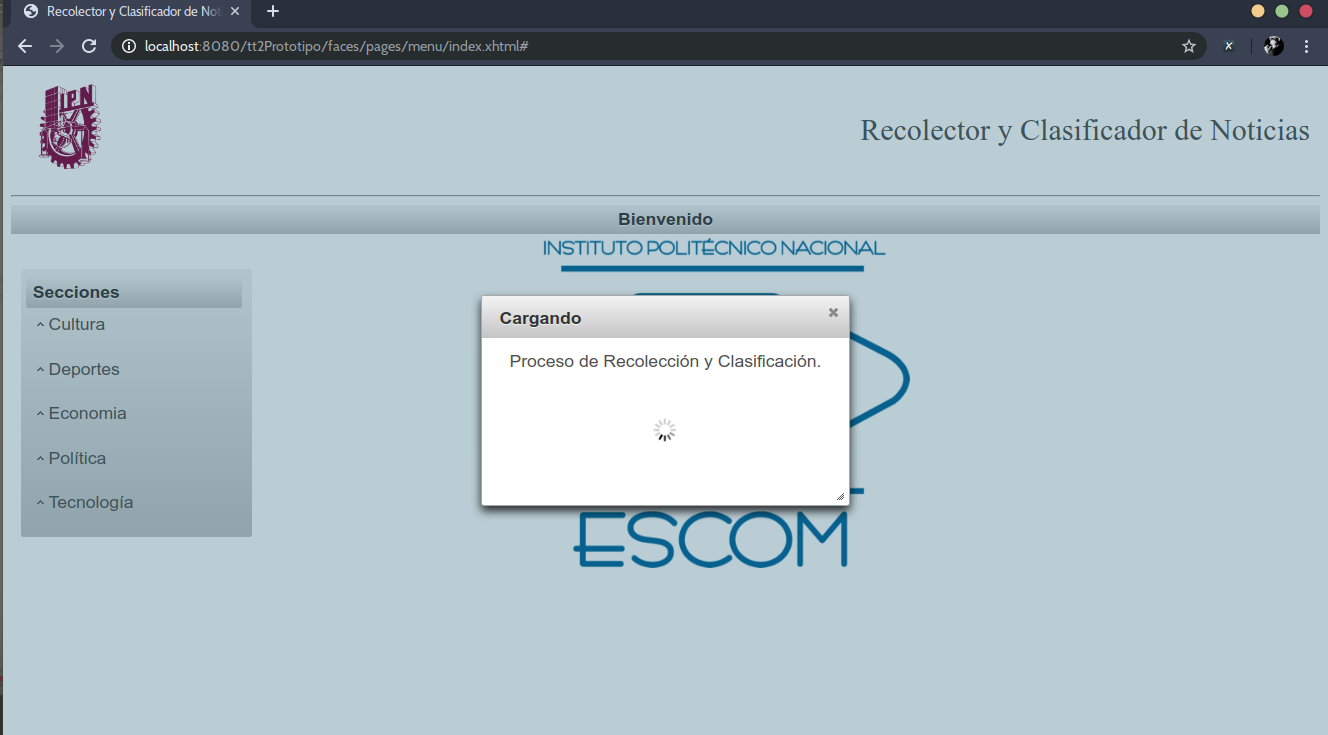
\includegraphics[scale=0.3]{imagenes/Aplicacion/seleccionarSeccion.png}
\caption{Mensaje de aplicación}
\label{fig:seleccionarSeccion}
\end{figure}

Al concluir el proceso se muestra un mensaje para notificar al usuario
que han sido clasificadas las noticias como se visualiza en la Figura \ref{fig:noticiasListas} y el usuario tiene la opción de continuar con el proceso o cancelarlo.\\

\begin{figure}[ht]
\centering
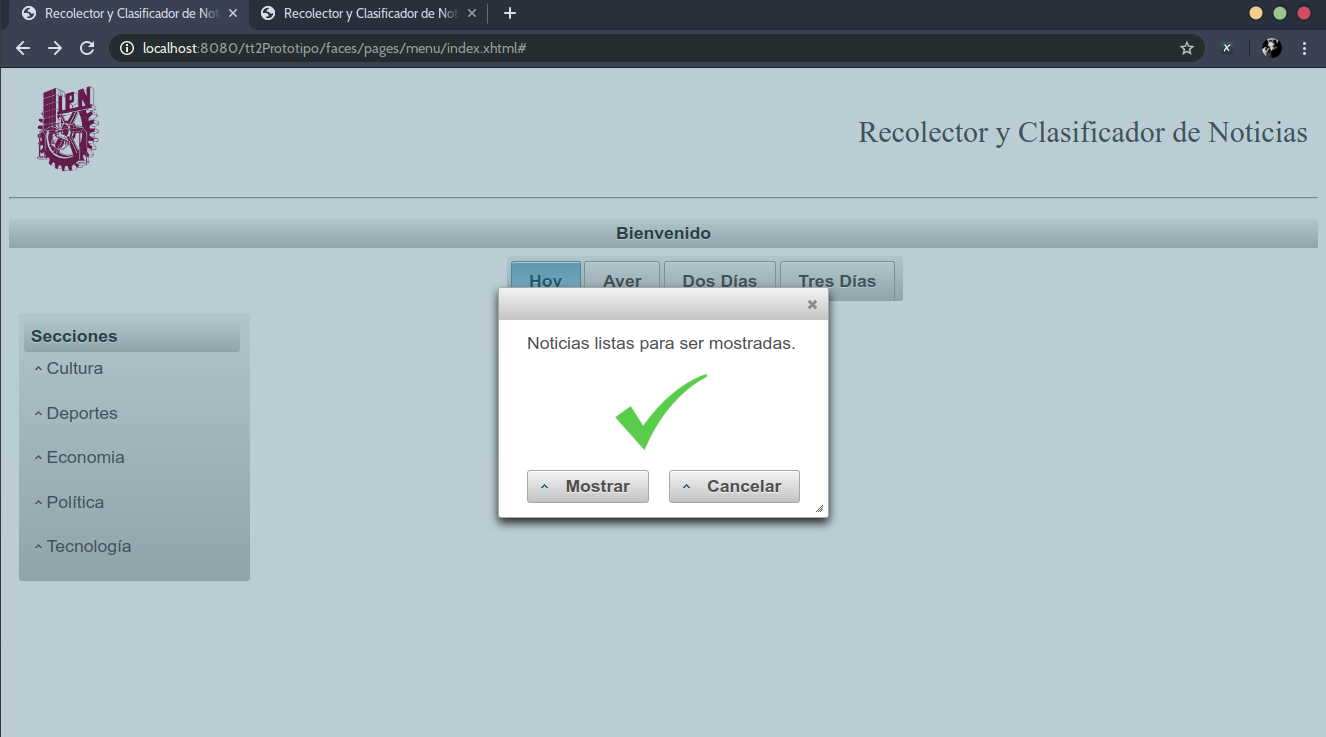
\includegraphics[scale=0.3]{imagenes/Aplicacion/noticiasListas.png}
\caption{Mensaje de aplicación}
\label{fig:noticiasListas}
\end{figure}

Si el usuario ha decidido continuar con el proceso de recolección y clasificación, la aplicación muestra las noticias de la sección seleccionada. Además se genera una menú en la parte superior de la pantalla en el cual el usuario puede filtrar las noticias en un periodo de tres días, como se visualiza en la Figura \ref{fig:mostrarNoticias}.\\
 
\begin{figure}[ht]
\centering
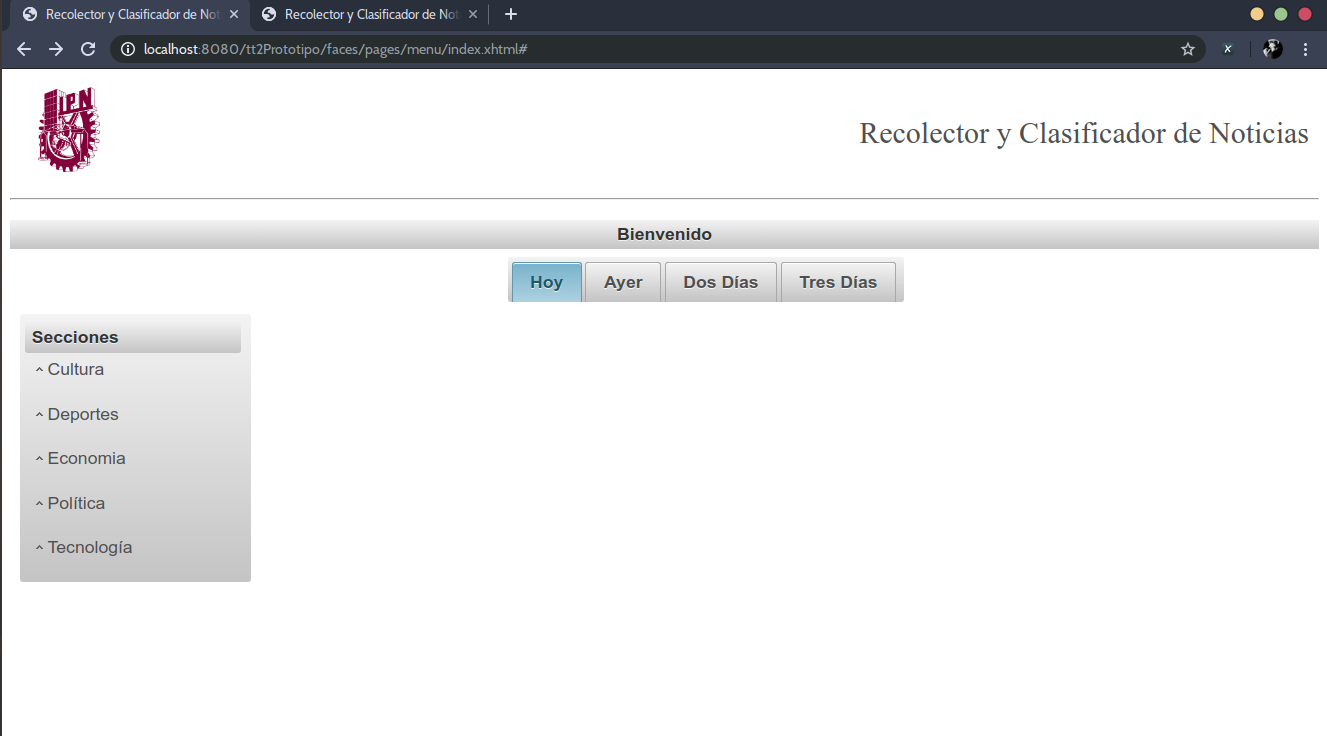
\includegraphics[scale=0.3]{imagenes/Aplicacion/mostrarNoticias.png}
\caption{Noticias clasificadas}
\label{fig:mostrarNoticias}
\end{figure}


\subsection{Backend}

Para el desarrollo de la aplicación web se ocupa un repositorio de \textit{Maven} el cual permite controlar las versiones de las dependencias así como de las librerías utilizadas.\\

La implementación del \textbf{Backend} se está programando en \textbf{Python} y \textbf{Javs server faces}.

\begin{itemize}
	\item \textbf{Python}: En este lenguaje de programación se está desarrollando el clasificador con la librería \textit{Scikt learn} y los \textit{Crawlers} con la librería \textit{Scrapy}.

	\item \textbf{Java server faces}: La interacción del usuario con la aplicación se va desarrollar en este \textit{framework}, y es en este punto donde se va programar la unión del proceso de clasificación y recolección con la aplicación web. Cabe destacar que esto aun no se ha iniciado debido a que los clasificadores siguen en pruebas.
\end{itemize}


